\section{Resultados}


\subsection{Promedio de Reconocimiento}
La m\'etodologia de implementaci\'on fue la siguiente: Se construy\'o una
m\'atriz de covarianza utilizando los primeros $n$ elementos del dataset
\texttt{Training Data}. Luego, se tomaron $t$ elementos siguientes como im\'agenes
de test, con sus correspondientes labels. A estos se les aplicaron las t\'ecnicas
de detecci\'on que hemos detallado antes y fuimos variando las $k$ cantidad de
columnas de las tuplas que tomabamos para hacer las cuentas de distancia.
Los gr\'aficos de HitRate est\'an hechos en funci\'on de $k$.

Testeamos usando matrices de covarianza entrenadas con cantidad variable de elementos.
\def \hrwidth {500pt}

\begin{figure}[H]
\begin {center}
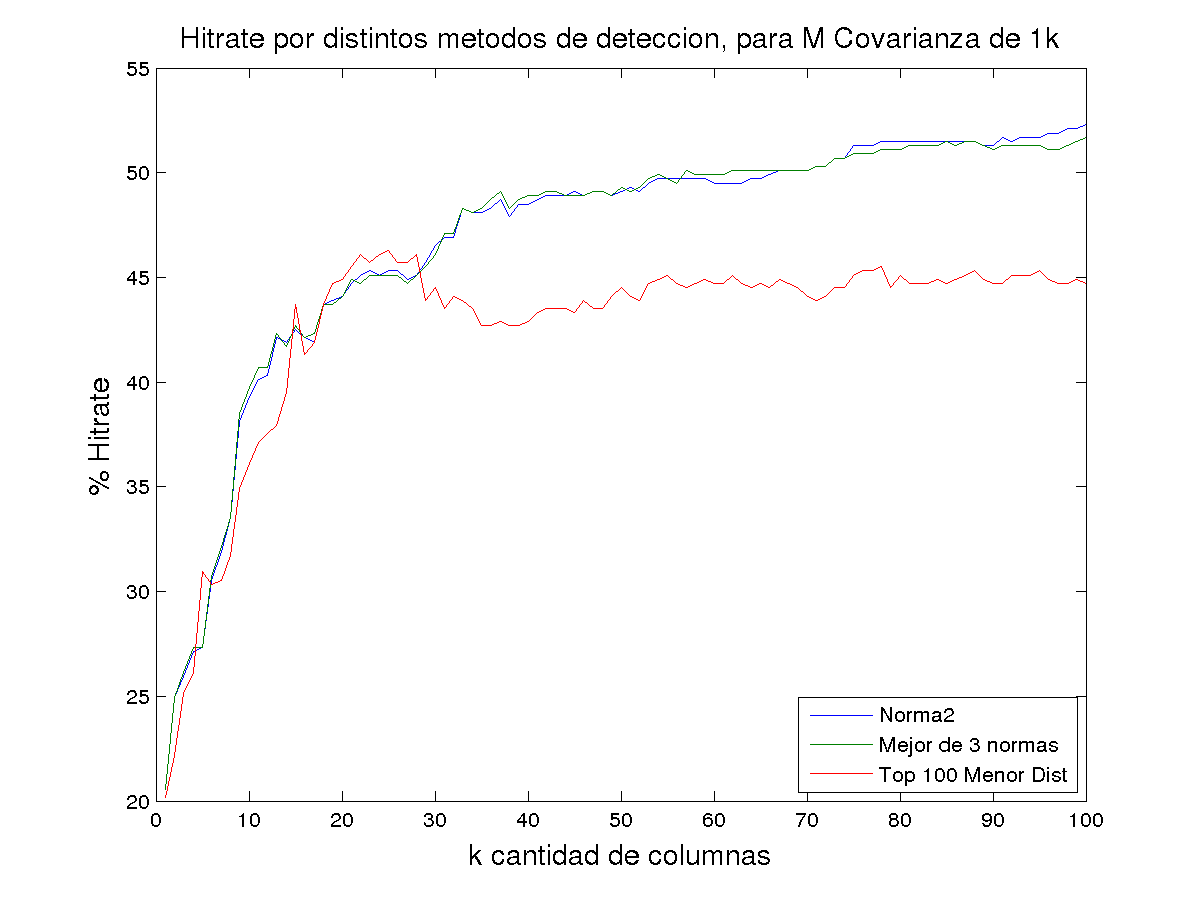
\includegraphics[width=\hrwidth]{plots/hitrate-1kcv.png}
\end {center}
\caption{Hitrate de detecci\'on de 500 elementos de acuerdo a los varios m\'etodos implementados
usando la matriz de covarianza entrenada con 1000 elementos}
\label{fig:HR1kcv}
\end{figure}

\begin{figure}[H]
\begin {center}
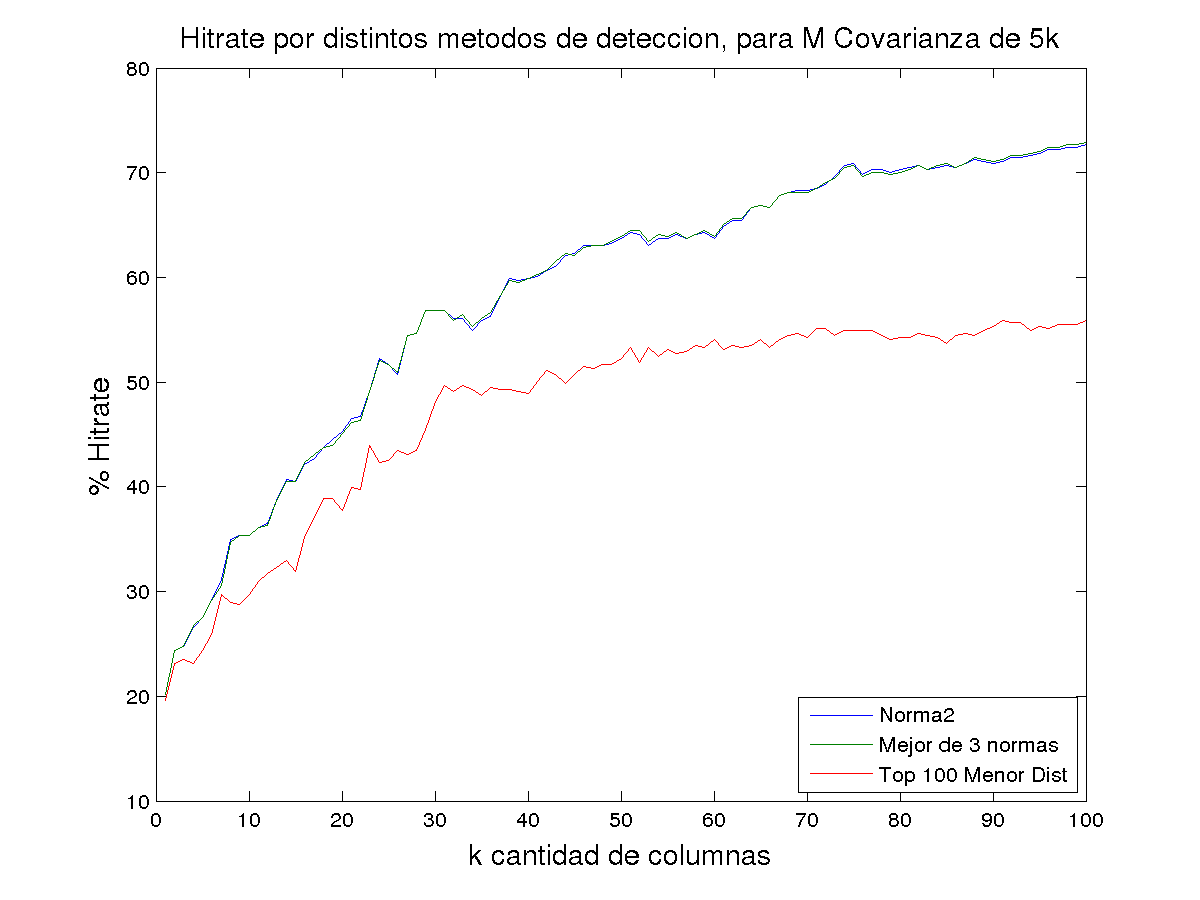
\includegraphics[width=\hrwidth]{plots/hitrate-5kcv.png}
\end {center}
\caption{Hitrate de detecci\'on de 500 elementos de acuerdo a los varios m\'etodos implementados
usando la matriz de covarianza entrenada con 5000 elementos}
\label{fig:HR5kcv}
\end{figure}

\begin{figure}[H]
\begin {center}
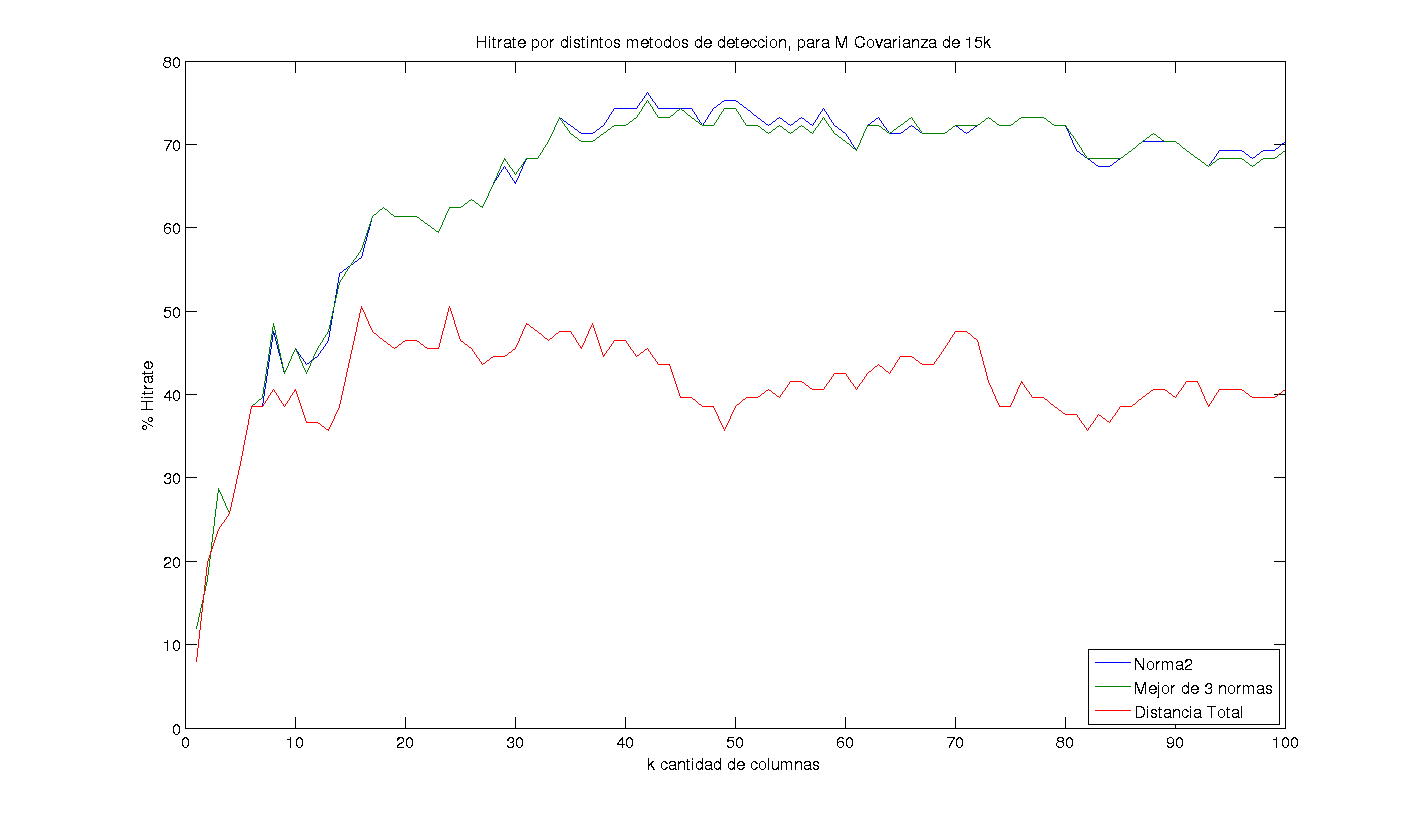
\includegraphics[width=\hrwidth]{plots/hitrate-15kcv.png}
\end {center}
\caption{Hitrate de detecci\'on de 500 elementos de acuerdo a los varios m\'etodos implementados
usando la matriz de covarianza entrenada con 15000 elementos}
\label{fig:HR15kcv}
\end{figure}

\begin{figure}[H]
\begin {center}
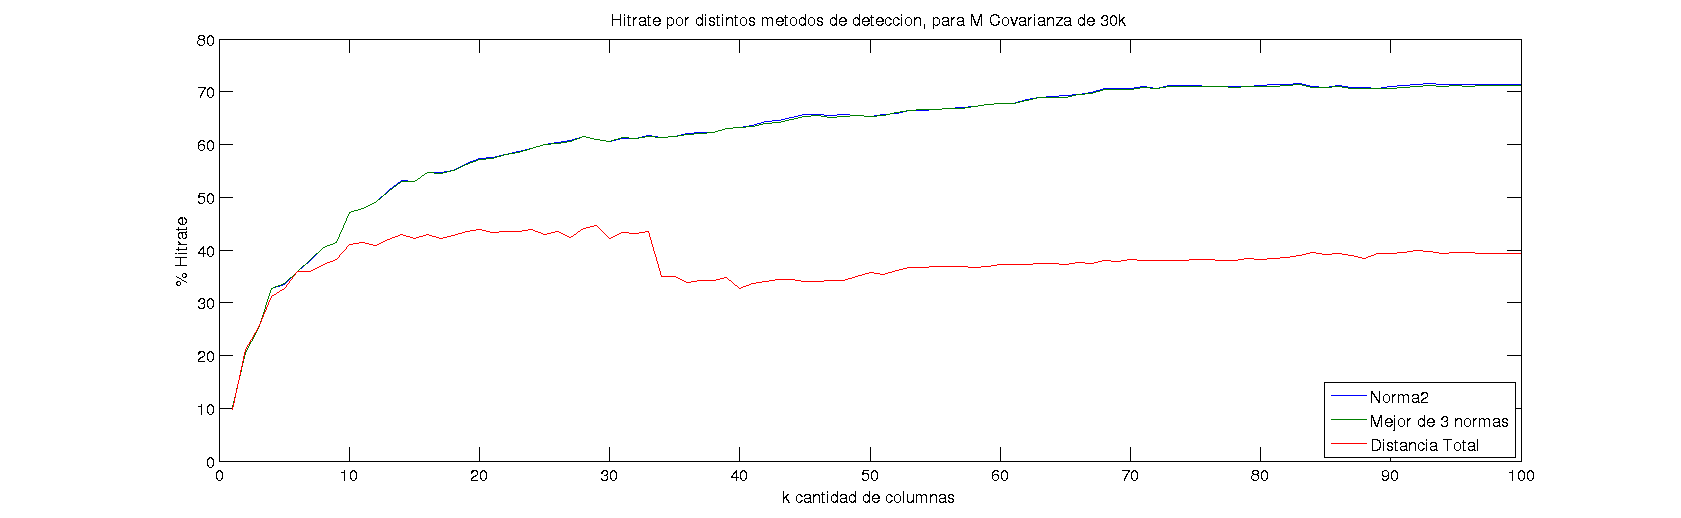
\includegraphics[width=\hrwidth]{plots/hitrate-30kcv.png}
\end {center}
\caption{Hitrate de detecci\'on de 500 elementos de acuerdo a los varios m\'etodos implementados
usando la matriz de covarianza entrenada con 30000 elementos}
\label{fig:HR30kcv}
\end{figure}



\subsection{Reconocimiento por d\'igito}
Fijamos la matriz de covarianza entrenada con 30000 elementos, ya que est\'a precalculada.
Siguiendo la misma metodologia, nos concentramos ahora en el HitRate individual
de cada d\'igito. Analizamos el HitRate de acuerdo a la metodolog\'ia de detecci\'on usada.
\def \pdwidth {500pt}

\begin{figure}[H]
\begin {center}
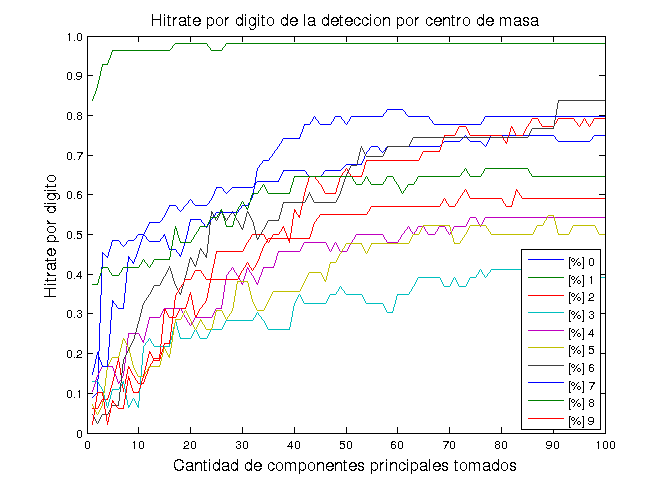
\includegraphics[width=\pdwidth]{plots/pordig-30kcv-norma2.png}
\end {center}
\caption{Hitrate por d\'igito de detecci\'on de 500 elementos usando la matriz de covarianza entrenada con 30000 elementos
clasificados por norma2}
\label{fig:HRD30kcv-n2}
\end{figure}

\begin{figure}[H]
\begin {center}
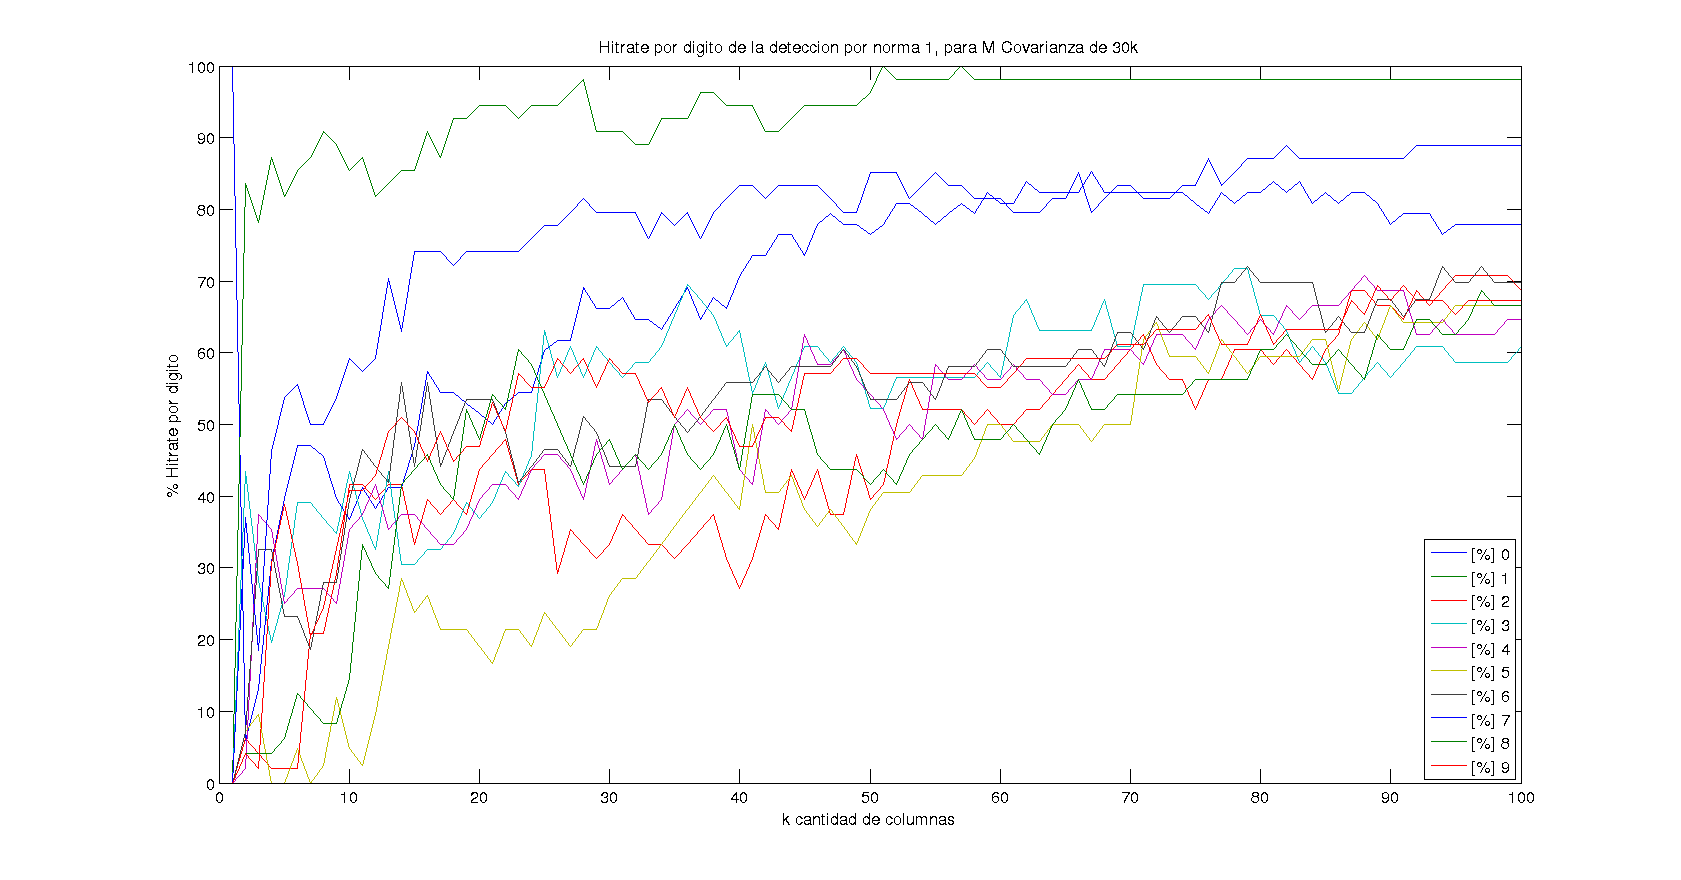
\includegraphics[width=\pdwidth]{plots/pordig-30kcv-norma1.png}
\end {center}
\caption{Hitrate por d\'igito de detecci\'on de 500 elementos usando la matriz de covarianza entrenada con 30000 elementos
clasificados por norma1}
\label{fig:HRD30kcv-n1}
\end{figure}

\begin{figure}[H]
\begin {center}
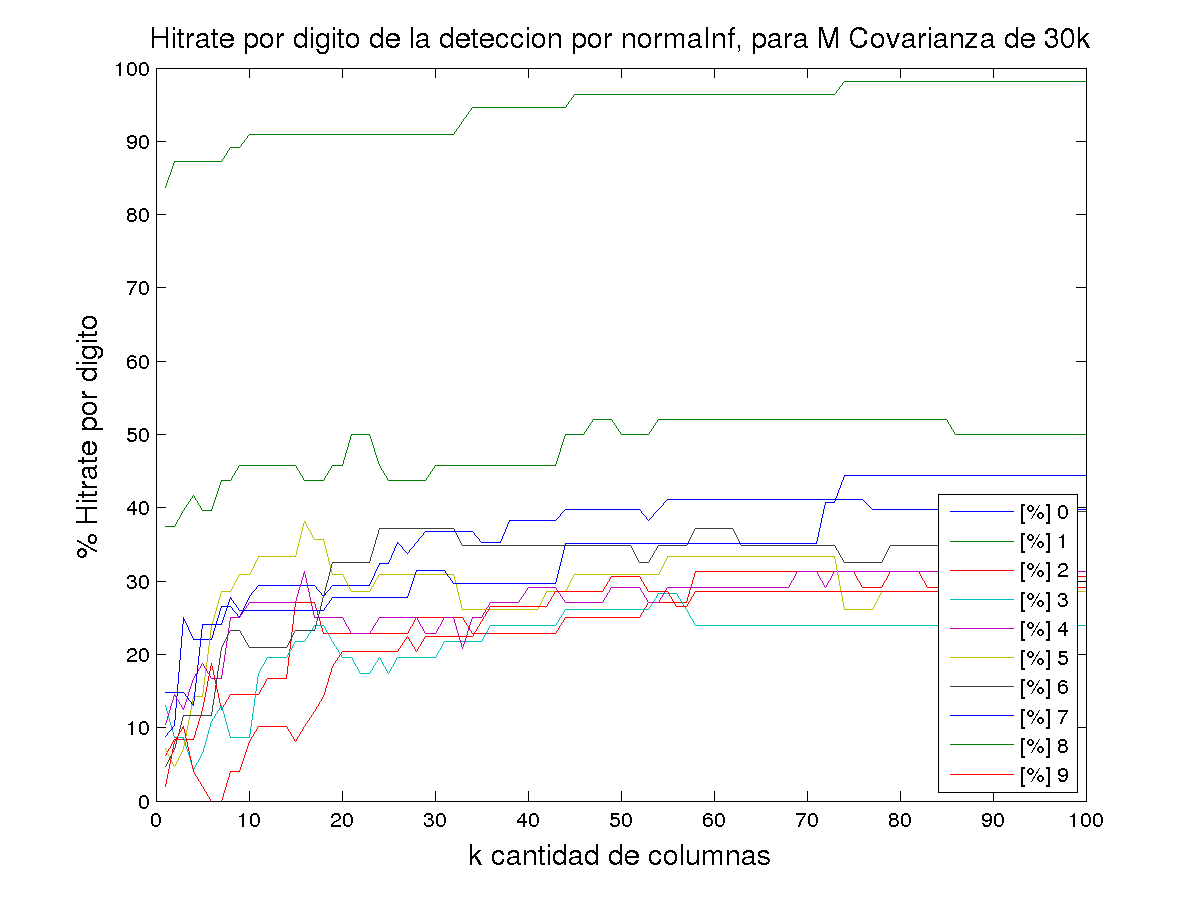
\includegraphics[width=\pdwidth]{plots/pordig-30kcv-normaInf.png}
\end {center}
\caption{Hitrate por d\'igito de detecci\'on de 500 elementos usando la matriz de covarianza entrenada con 30000 elementos
clasificados por norma Inf}
\label{fig:HRD30kcv-ninf}
\end{figure}

\begin{figure}[H]
\begin {center}
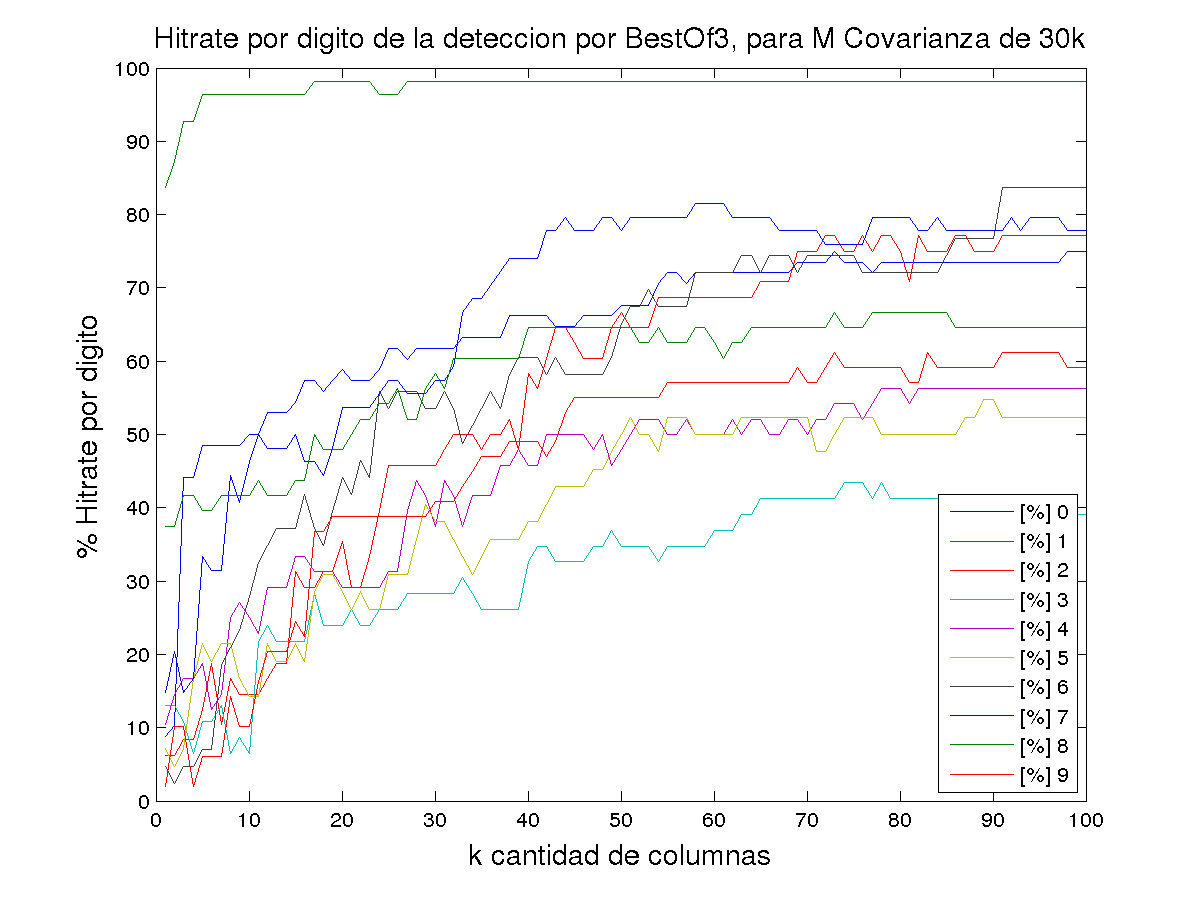
\includegraphics[width=\pdwidth]{plots/pordig-30kcv-BestOf3.png}
\end {center}
\caption{Hitrate por d\'igito de detecci\'on de 500 elementos usando la matriz de covarianza entrenada con 30000 elementos
clasificados por mejor de 3 normas}
\label{fig:HRD30kcv-bo3}
\end{figure}

\begin{figure}[H]
\begin {center}
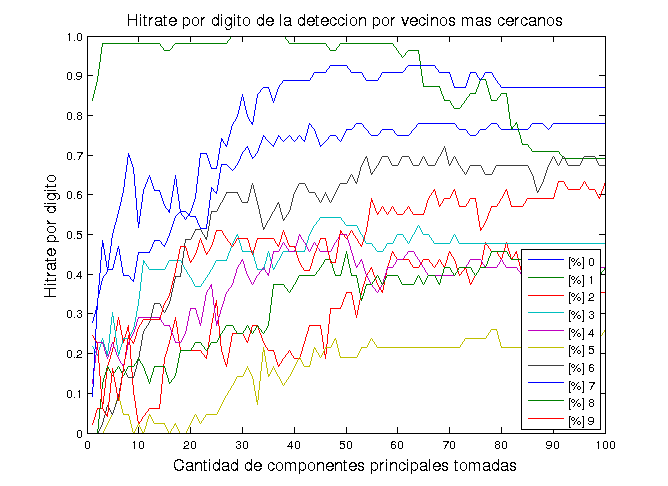
\includegraphics[width=\pdwidth]{plots/pordig-30kcv-top100.png}
\end {center}
\caption{Hitrate por d\'igito de detecci\'on de 500 elementos usando la matriz de covarianza entrenada con 30000 elementos
clasificados por distancia a 100 m\'as cercanos}
\label{fig:HRD30kcv-dist100}
\end{figure}

\section{Heatmap de reconocimiento por d\'igito}
Aca mostramos las equivocaciones y aciertos al reconocer cada d\'igito, variando la cantidad de columnas, hecho con la matriz de covarianza de
30000 elementos y variando la cantidad de columnas tomadas. Eje X el valor detectado, eje Y el valor verdadero. El color marca la cantidad
de veces que se detect\'o un valor y a cual correspondia.
\def \hmwidth {500pt}
\begin{figure}[H]
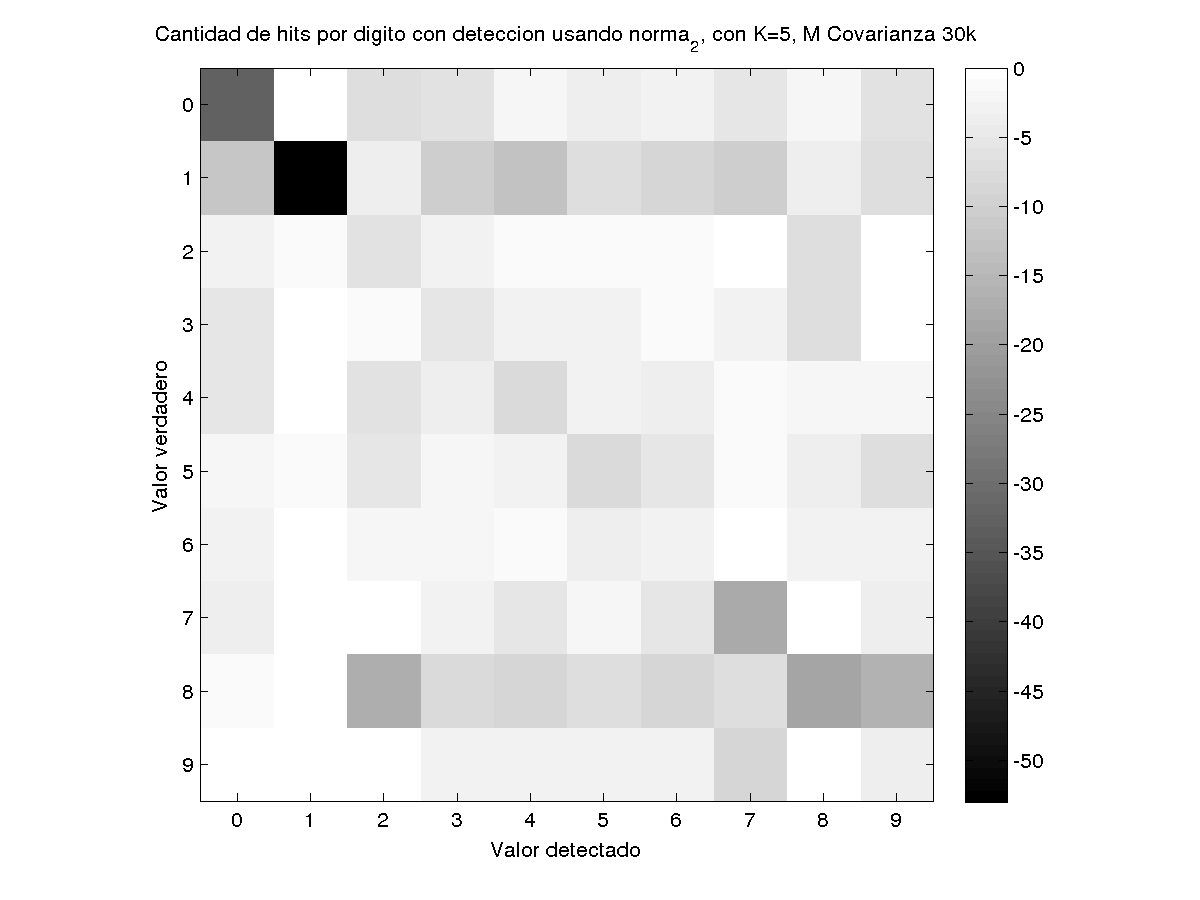
\includegraphics[width=\hmwidth]{plots/heatmap-30kcv-k5-norma_2.png}
\caption{Heatmap de aciertos por d\'igito de detecci\'on de 500 elementos usando la matriz de covarianza entrenada con 30000 elementos
clasificados por norma 2 tomando K=5}
\label{fig:HM30kcv-k5}
\end{figure}

\begin{figure}[H]
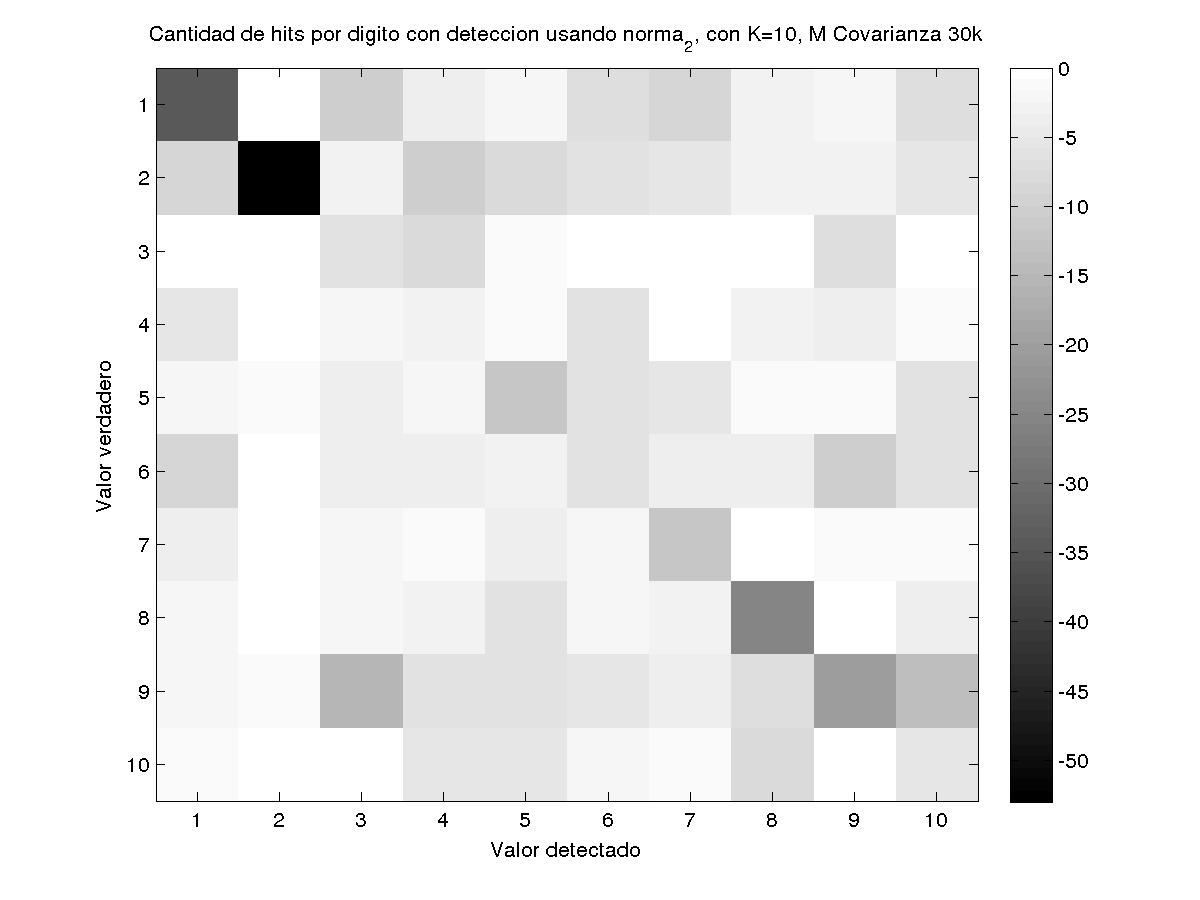
\includegraphics[width=\hmwidth]{plots/heatmap-30kcv-k10-norma_2.png}
\caption{Heatmap de aciertos por d\'igito de detecci\'on de 500 elementos usando la matriz de covarianza entrenada con 30000 elementos
clasificados por norma 2 tomando K=10 }
\label{fig:HM30kcv-k10}
\end{figure}

\begin{figure}[H]
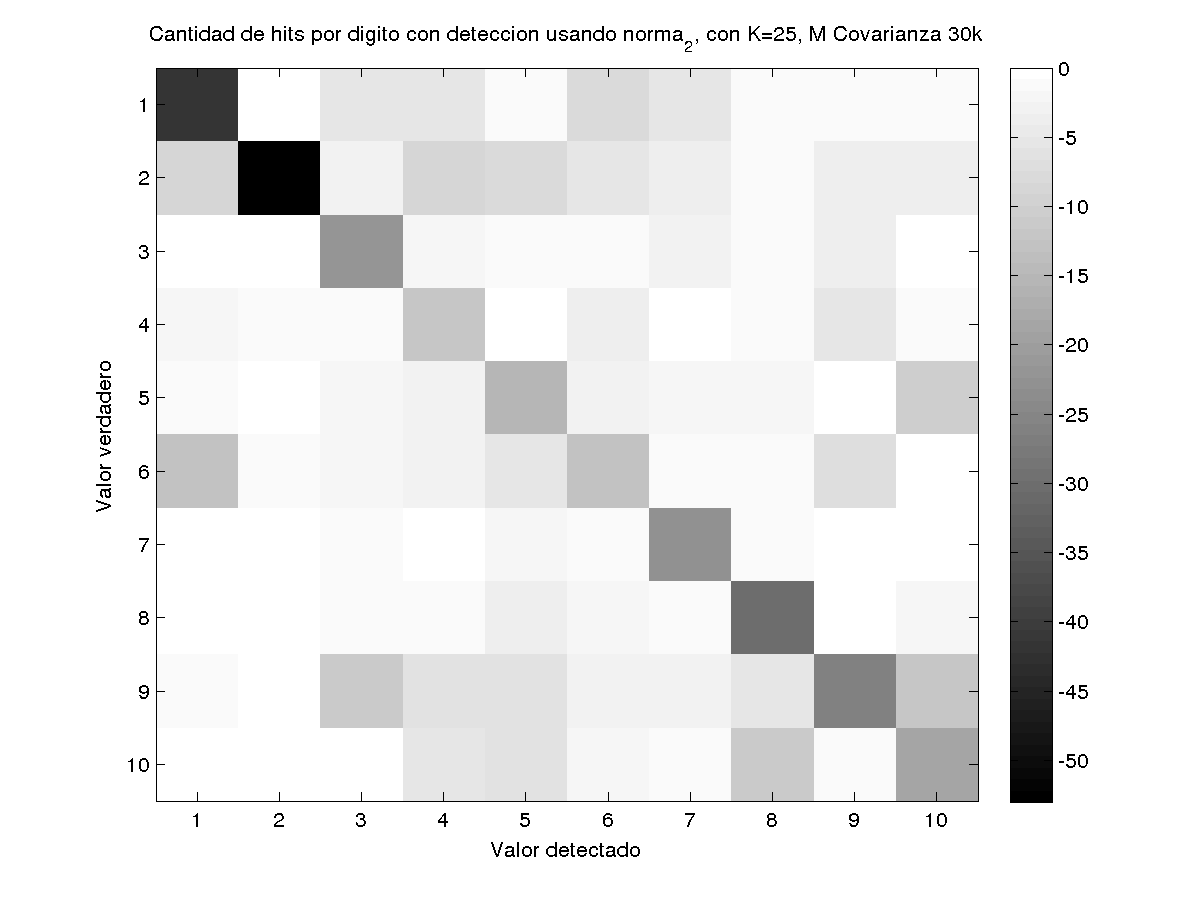
\includegraphics[width=\hmwidth]{plots/heatmap-30kcv-k25-norma_2.png}
\caption{Heatmap de aciertos por d\'igito de detecci\'on de 500 elementos usando la matriz de covarianza entrenada con 30000 elementos
clasificados por norma 2 tomando K=25 }
\label{fig:HM30kcv-k25}
\end{figure}

\begin{figure}[H]
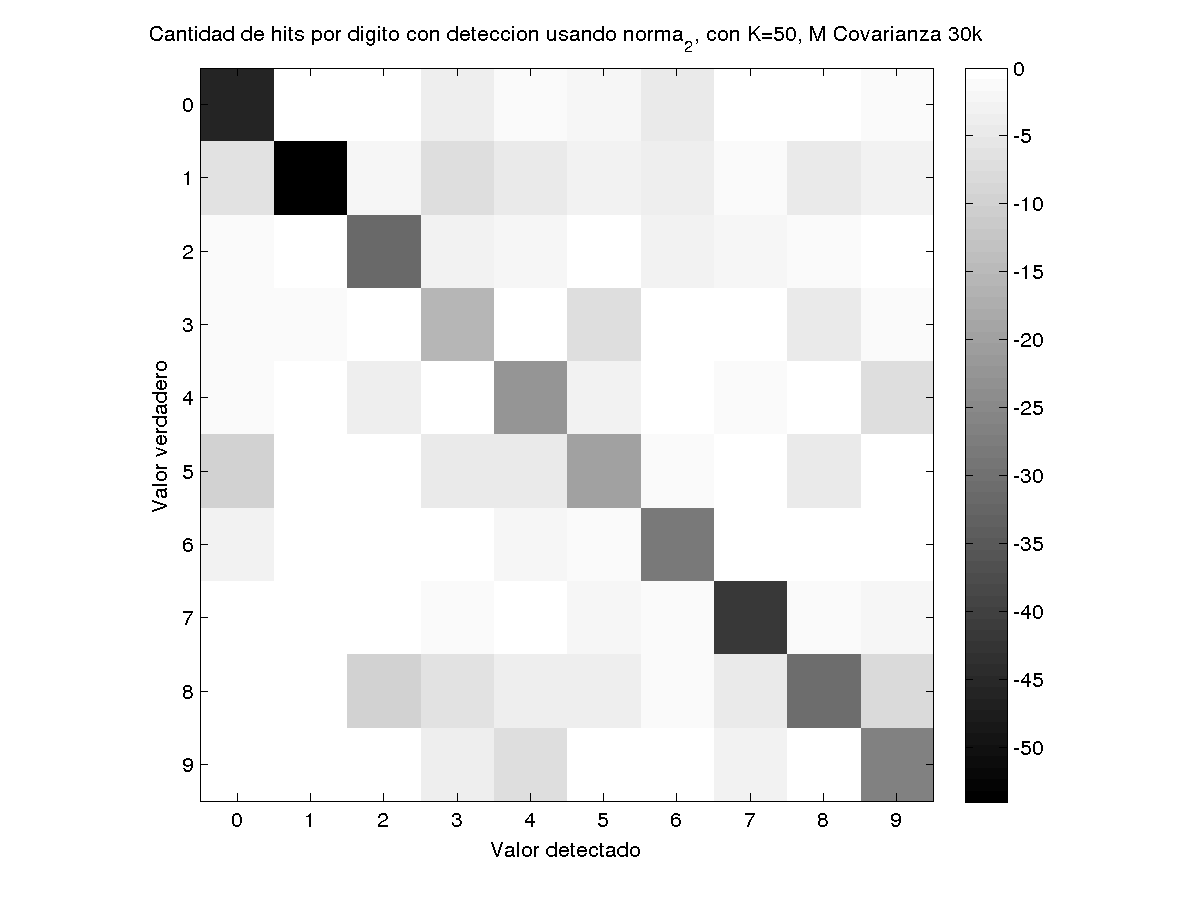
\includegraphics[width=\hmwidth]{plots/heatmap-30kcv-k50-norma_2.png}
\caption{Heatmap de aciertos por d\'igito de detecci\'on de 500 elementos usando la matriz de covarianza entrenada con 30000 elementos
clasificados por norma 2 tomando K=50 }
\label{fig:HM30kcv-k50}
\end{figure}
